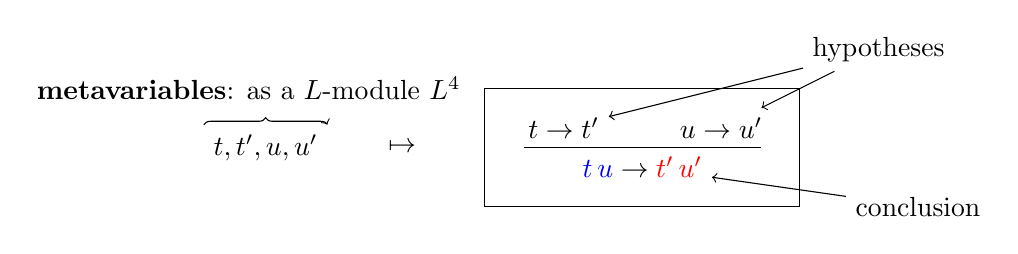
\begin{tikzpicture}[->]


\draw[-] (-4,2.75) -- (-1,2.75);

\node (v8) at (-3.5,3) {$t\rightarrow t'$};
\node (v9) at (-1.5,3) {$u\rightarrow u'$}; 
\node (v11) at (-2.5,2.5) {${\color{blue}t\,u}\rightarrow{\color{red}t'\,u'}$};
\draw  (-4.5,3.5) rectangle (-0.5,2);
\node (v7) at (0.5,4) {hypotheses};
\node (v10) at (1,2) {conclusion};
\draw  (v7) edge (v8);
\draw  (v7) edge (v9);
\draw  (v10) edge (v11);
% \node[anchor=west] at (1,3) {metavariables: $t,t',u,u'$};
% \node[anchor=west] at (1,2.5) {$\Rightarrow$ as a $L$-module: $L^4$};
\node[anchor=east] (mv) at (-6.5,2.75) {$t,t',u,u'$};
\draw[decorate, decoration = brace] (mv.north west) -- (mv.north east);
% \node[midway, above] {metavariables};
\node[anchor=east] at (-5.25,2.75) {$\mapsto$};
\node at (-7.5,3.5) {\textbf{metavariables}: as a $L$-module $L^4$};
\end{tikzpicture}
